\mainmatter
\chapter{Introduction}





\section{High-Energy Particle Physics and Standard Model}
Understanding the nature of the particles that constitute matter and radiation is one of the main concerns of science. Particle Physics, also known as High-Energy Physics (briefly, "hep"), is the branch of Physics that conducts this ambitious research and its development can be located near the end of $19^\mathrm{th}$ century. Since then numerous theoretical models have been built in order to predict the outcome of experiments, which can prove their correctness.

At the present, the model that better describes the observed phenomena in hep is the Standard Model, which will be identified with the acronym SM. Since it is the best basis for comparison with experimental results, it will be denoted as reference model in the following discussion. 

\begin{figure}[H]
	\centering
	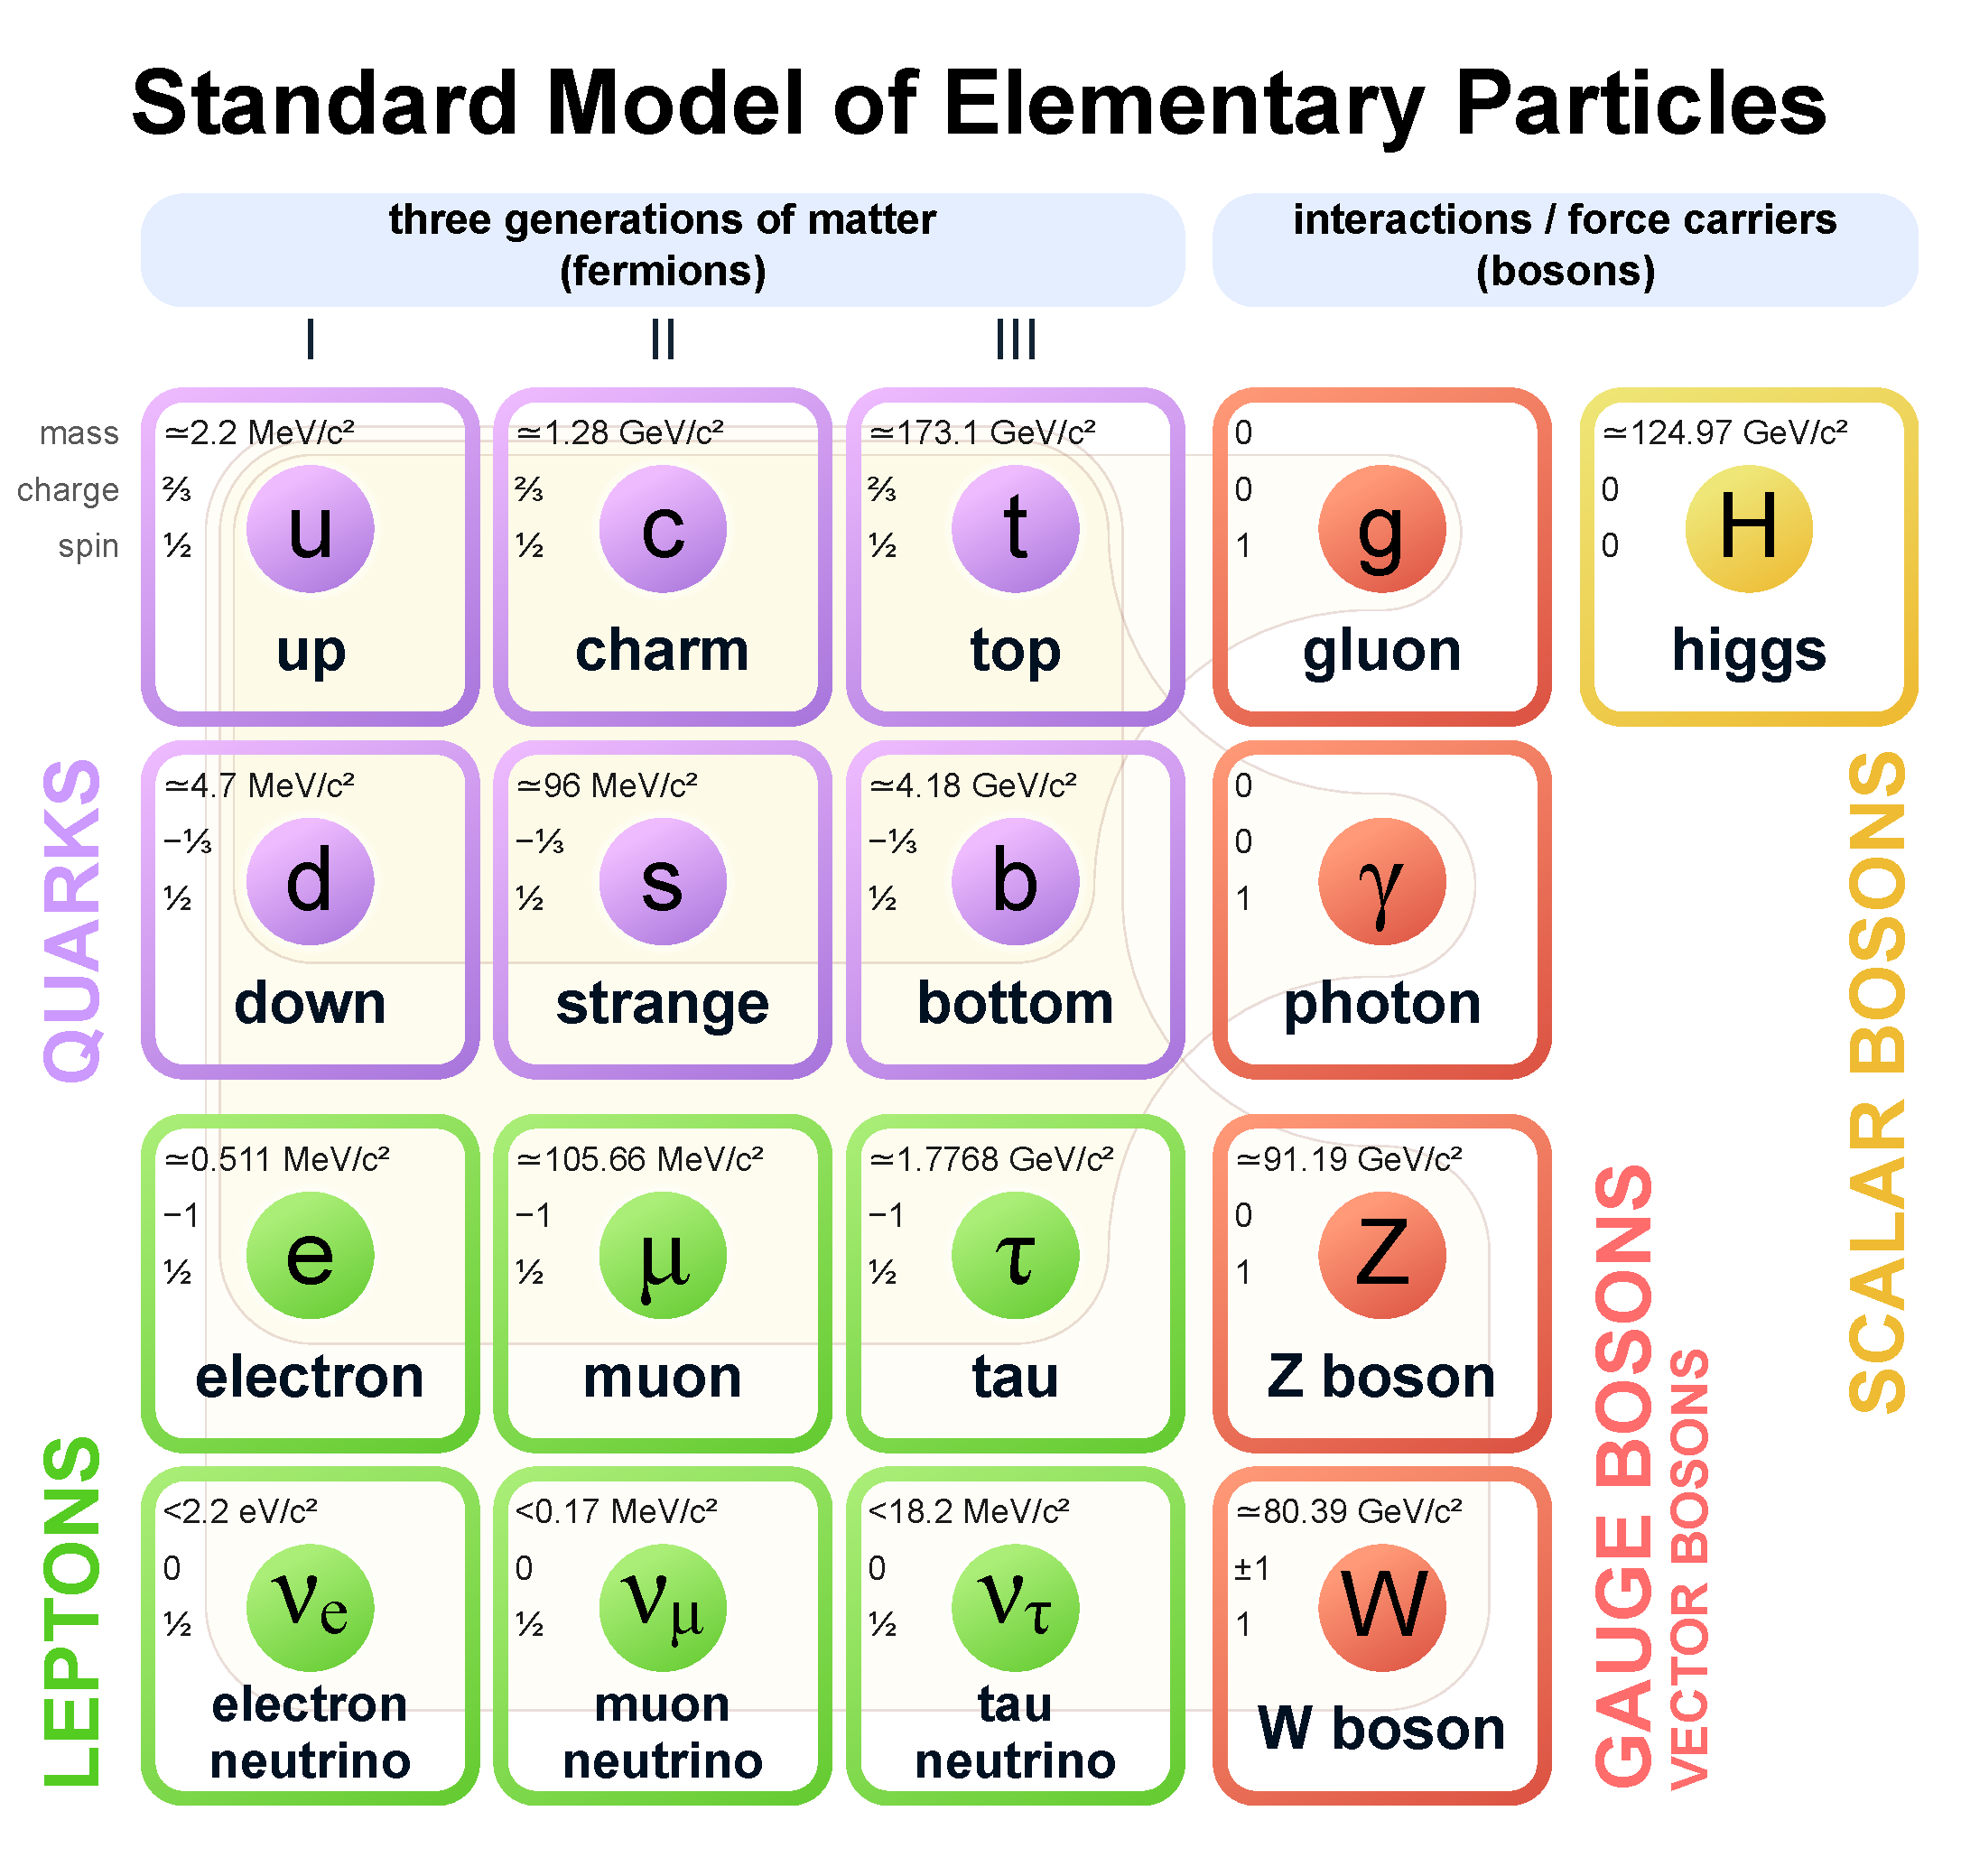
\includegraphics[width=0.4\textwidth]{Images/Introduction/SM_particles.pdf}
	\caption{Standard Model particles.}
	\label{fig:SM_PARTICLES}
\end{figure}

\noindent
However, althought SM has proved to be extremely successful in predicting a wide variety of particle processes with great accuracy, there are still unexplained phenomena. Among these:
\begin{itemize}
    \item It doesn't explain the canonical theory of gravitation, general relativity, in terms of quantum field theory\footnotemark.
    \footnotetext{It is important to remark that an eventual physical confirmation of a theoretical particle known as a graviton would account for it to a degree.}
    \item Although, as it now stands, it can explain why neutrinos have masses, the specifics of neutrino mass are still unclear.
    \item It doesn't explain the existence of dark matter.
\end{itemize}
Future experiments will be able to explore never observed before phenomena, or they will mesaure known phenomena with a even better accuracy. These facts suggest that new physics (i.e. physical laws not yet established) exists and its research is actually one of the most challenging problems in High-Energy Physics.



\subsection{Researches for new physics}
Searching for new physics concretely means searching for discrepancies between observed data and reference model. This task can be phrased in a more technical way. What we are able to do is taking repeated measurements of a multi-dimensional random variable $x$, experimentally speaking. Then, we can build a Probability Density Function (PDF) using experimental data and test the reference model distribution against the actual data. The first difficulty encountered by seeking this approach is that the true underlying data distribution will be quite similar to the reference one. It means that, if data contain new physics effects, they will be localized in a low-probability region where only a small fraction of event is present, or they will be spread in a large region of the $x$ space.

The most widely employed approach to the problem is to search for specific new physics models. It has the advantage to be physically informative, even if the compatibility of the data with the reference model is confirmed. But there is a critical disadvantage: a statistical test which is designed to be sensitive to one specific hypothesis is typically insensitive to data departures of a different nature from the one expected. So, even if new physics is present in the data, it would not be discovered because it doesn't belong to the class of hypothetical models we are searching for.



\subsection{The need for a model-independent approach}
It is necessary to define the meaning of 'model-independent'. We call a certain approach 'model-independent' when the alternative distributions don't follow from a physical model, but are selected with other criteria, such as flexibility. It means that the distributions can adapt to the true underlying data distribution for an appropriate choice of the free parameters.

The main reason for which we demand a model-independent approach is the advantage of sensitivity to a large variety of new physics scenarios, including those that are not predicted by any of the models constructed until now.





\section{Why do we choose Neural Networks?}
Neural Networks are increasing their importance in high energy physics since they are widely employed. The main reason for their success is due to their properties of unbiased approximants. In fact, it is possible to prove mathematically that a Network of a certain complexity can approximate every function sufficiently regular. Employing them to parametrize alternative distributions for model-independent new physics searches is thus a highly motivated attempt.

Technically speaking, we can exploit Neural Networks to find an anomalous behavior, relative to the reference model, of the entire data sample with which we train the Network.